\documentclass[12pt]{article}
\usepackage[letterpaper,margin=1in]{geometry}
\usepackage{graphicx}
\usepackage{xcolor}
\usepackage{hyperref}
\usepackage{array}
\usepackage{booktabs}
\usepackage{float}
\usepackage{verbatim}

\graphicspath{{assets/}}
\hypersetup{colorlinks=true,linkcolor=black,urlcolor=blue}
\urlstyle{same}
\setlength{\parindent}{0pt}
\setlength{\parskip}{0.85em}
\renewcommand{\arraystretch}{1.18}

\definecolor{sectionred}{RGB}{220,38,38}
\definecolor{subblue}{RGB}{37,99,235}
\definecolor{softgray}{RGB}{245,247,250}

\newcommand{\majorsection}[1]{\clearpage\begin{center}{\LARGE\color{sectionred}#1}\end{center}\vspace{0.5em}}
\newcommand{\bluesubsection}[1]{\vspace{0.8em}{\Large\color{subblue}#1}\par\vspace{0.2em}}
\newcommand{\flowbox}[1]{\fbox{\begin{minipage}{0.62\linewidth}\centering\strut #1\strut\end{minipage}}}

\begin{document}

\begin{titlepage}
\centering
\vspace*{0.4in}
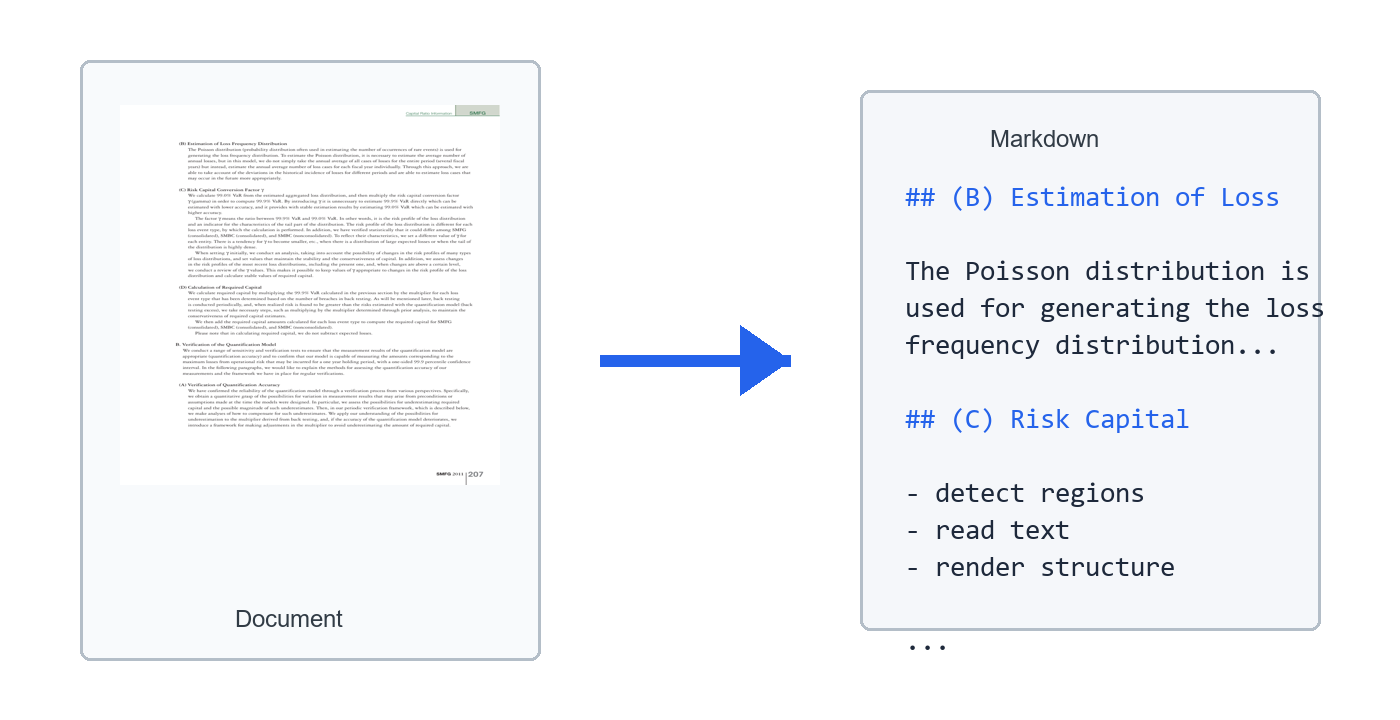
\includegraphics[width=0.92\textwidth,height=0.42\textheight,keepaspectratio]{cover_document_to_markdown.png}
\vfill
{\Huge Document-to-Markdown Reconstruction\par}
\vspace{0.35in}
{\Large using YOLO Layout Detection and PP-OCRv6 Recognition\par}
\vspace{0.25in}
{\large CAP 6665\par}
{\large Project 1\par}
\vfill
{\large Connor Austin\par}
{\large June 22, 2026\par}
\end{titlepage}

\majorsection{1) Description}

\bluesubsection{Description}

This project builds a computer vision pipeline that converts scanned or image-based document pages into structured Markdown. The goal is not only to read text from a page, but to preserve enough document structure that the output remains useful for archival, search, indexing, and downstream text processing.

A good document reconstruction system must satisfy four practical criteria:

\begin{enumerate}
  \item Semantic regions such as titles, section headers, paragraphs, lists, tables, pictures, captions, page headers, and footers should be detected correctly.
  \item The detected regions should be ordered in the same sequence a human reader would follow.
  \item OCR should read each text-bearing region accurately enough to preserve the meaning of the source page.
  \item Markdown rendering should preserve document structure with headings, paragraphs, lists, table approximations, figures, captions, and page metadata.
\end{enumerate}

The implemented system uses YOLO for document layout detection and PP-OCRv6 medium recognition for text extraction. YOLO is responsible for finding semantic page regions. OCR is only applied after those regions are cropped, which keeps detection and recognition as separate, testable stages. The final stages sort regions geometrically and convert them into Markdown.

\bluesubsection{Dataset and Classes}

The detector is trained on a DocLayNet-derived document layout dataset converted into YOLO format. The class set contains eleven document region types: Caption, Footnote, Formula, List-item, Page-footer, Page-header, Picture, Section-header, Table, Text, and Title. The data conversion scripts create separate detection and segmentation datasets so that both rectangular layout detection and mask-based experiments can be trained from the same source annotations.

\bluesubsection{Final Pipeline}

The final pipeline used for the demo is:

\begin{center}
\flowbox{Input scanned page}\\[0.4em]
$\downarrow$\\[0.4em]
\flowbox{YOLOv26m layout detection}\\[0.4em]
$\downarrow$\\[0.4em]
\flowbox{Crop each detected text region}\\[0.4em]
$\downarrow$\\[0.4em]
\flowbox{PP-OCRv6 medium recognition}\\[0.4em]
$\downarrow$\\[0.4em]
\flowbox{Geometry-based reading order}\\[0.4em]
$\downarrow$\\[0.4em]
\flowbox{Markdown reconstruction}
\end{center}

The repository packages the final YOLO checkpoints and the OCR recognition model so the grader can clone the repository, run the included setup script, and start the demo without downloading model weights or using a Hugging Face token.

\majorsection{2) Results and Analysis}

\bluesubsection{Detection Results}

The strongest packaged model is the YOLOv26m detection checkpoint trained for 20 epochs at 1024 pixel image size, batch size 8, using 20\% of the training data. Validation was run separately on the validation split. This model is used by default in the demo because it gives the best balance of layout quality, speed, and OCR compatibility.

\begin{center}
\begin{tabular}{>{\raggedright\arraybackslash}p{0.36\linewidth}cccc}
\toprule
Model & Precision & Recall & mAP50 & mAP50-95 \\
\midrule
YOLOv26m detection final & 0.869 & 0.825 & 0.884 & 0.724 \\
YOLOv26m detection prototype & 0.552 & 0.481 & 0.527 & 0.338 \\
YOLOv26m segmentation prototype, boxes & 0.537 & 0.501 & 0.532 & 0.355 \\
YOLOv26m segmentation prototype, masks & 0.527 & 0.494 & 0.519 & 0.345 \\
\bottomrule
\end{tabular}
\end{center}

The final detection model substantially outperformed the early detection and segmentation prototypes. Segmentation remains useful as an optional path when masks are needed, but for this project the rectangle detector was the better default because it gave stronger validation metrics and simpler OCR crops.

\bluesubsection{Analysis}

The final detector performs best on frequent structural classes such as Text, Table, Page-footer, Caption, Picture, and Section-header. The precision-recall curve shows strong overall behavior with all-class mAP50 of 0.884. The normalized confusion matrix shows that the main remaining mistakes are between visually similar document elements, especially text-like regions and background or header/footer material.

OCR quality depends heavily on the crop passed to PP-OCRv6. Because the packaged Paddle model is a recognition model rather than a full text detector, the pipeline splits YOLO crops into lines and chunks before recognition. This works well for normal paragraphs and headings, but special symbols, low-resolution text, and table ruling lines can still reduce OCR quality. The implementation therefore removes long table ruling lines before OCR splitting and reconstructs tables from OCR line geometry when possible.

\begin{figure}[H]
\centering
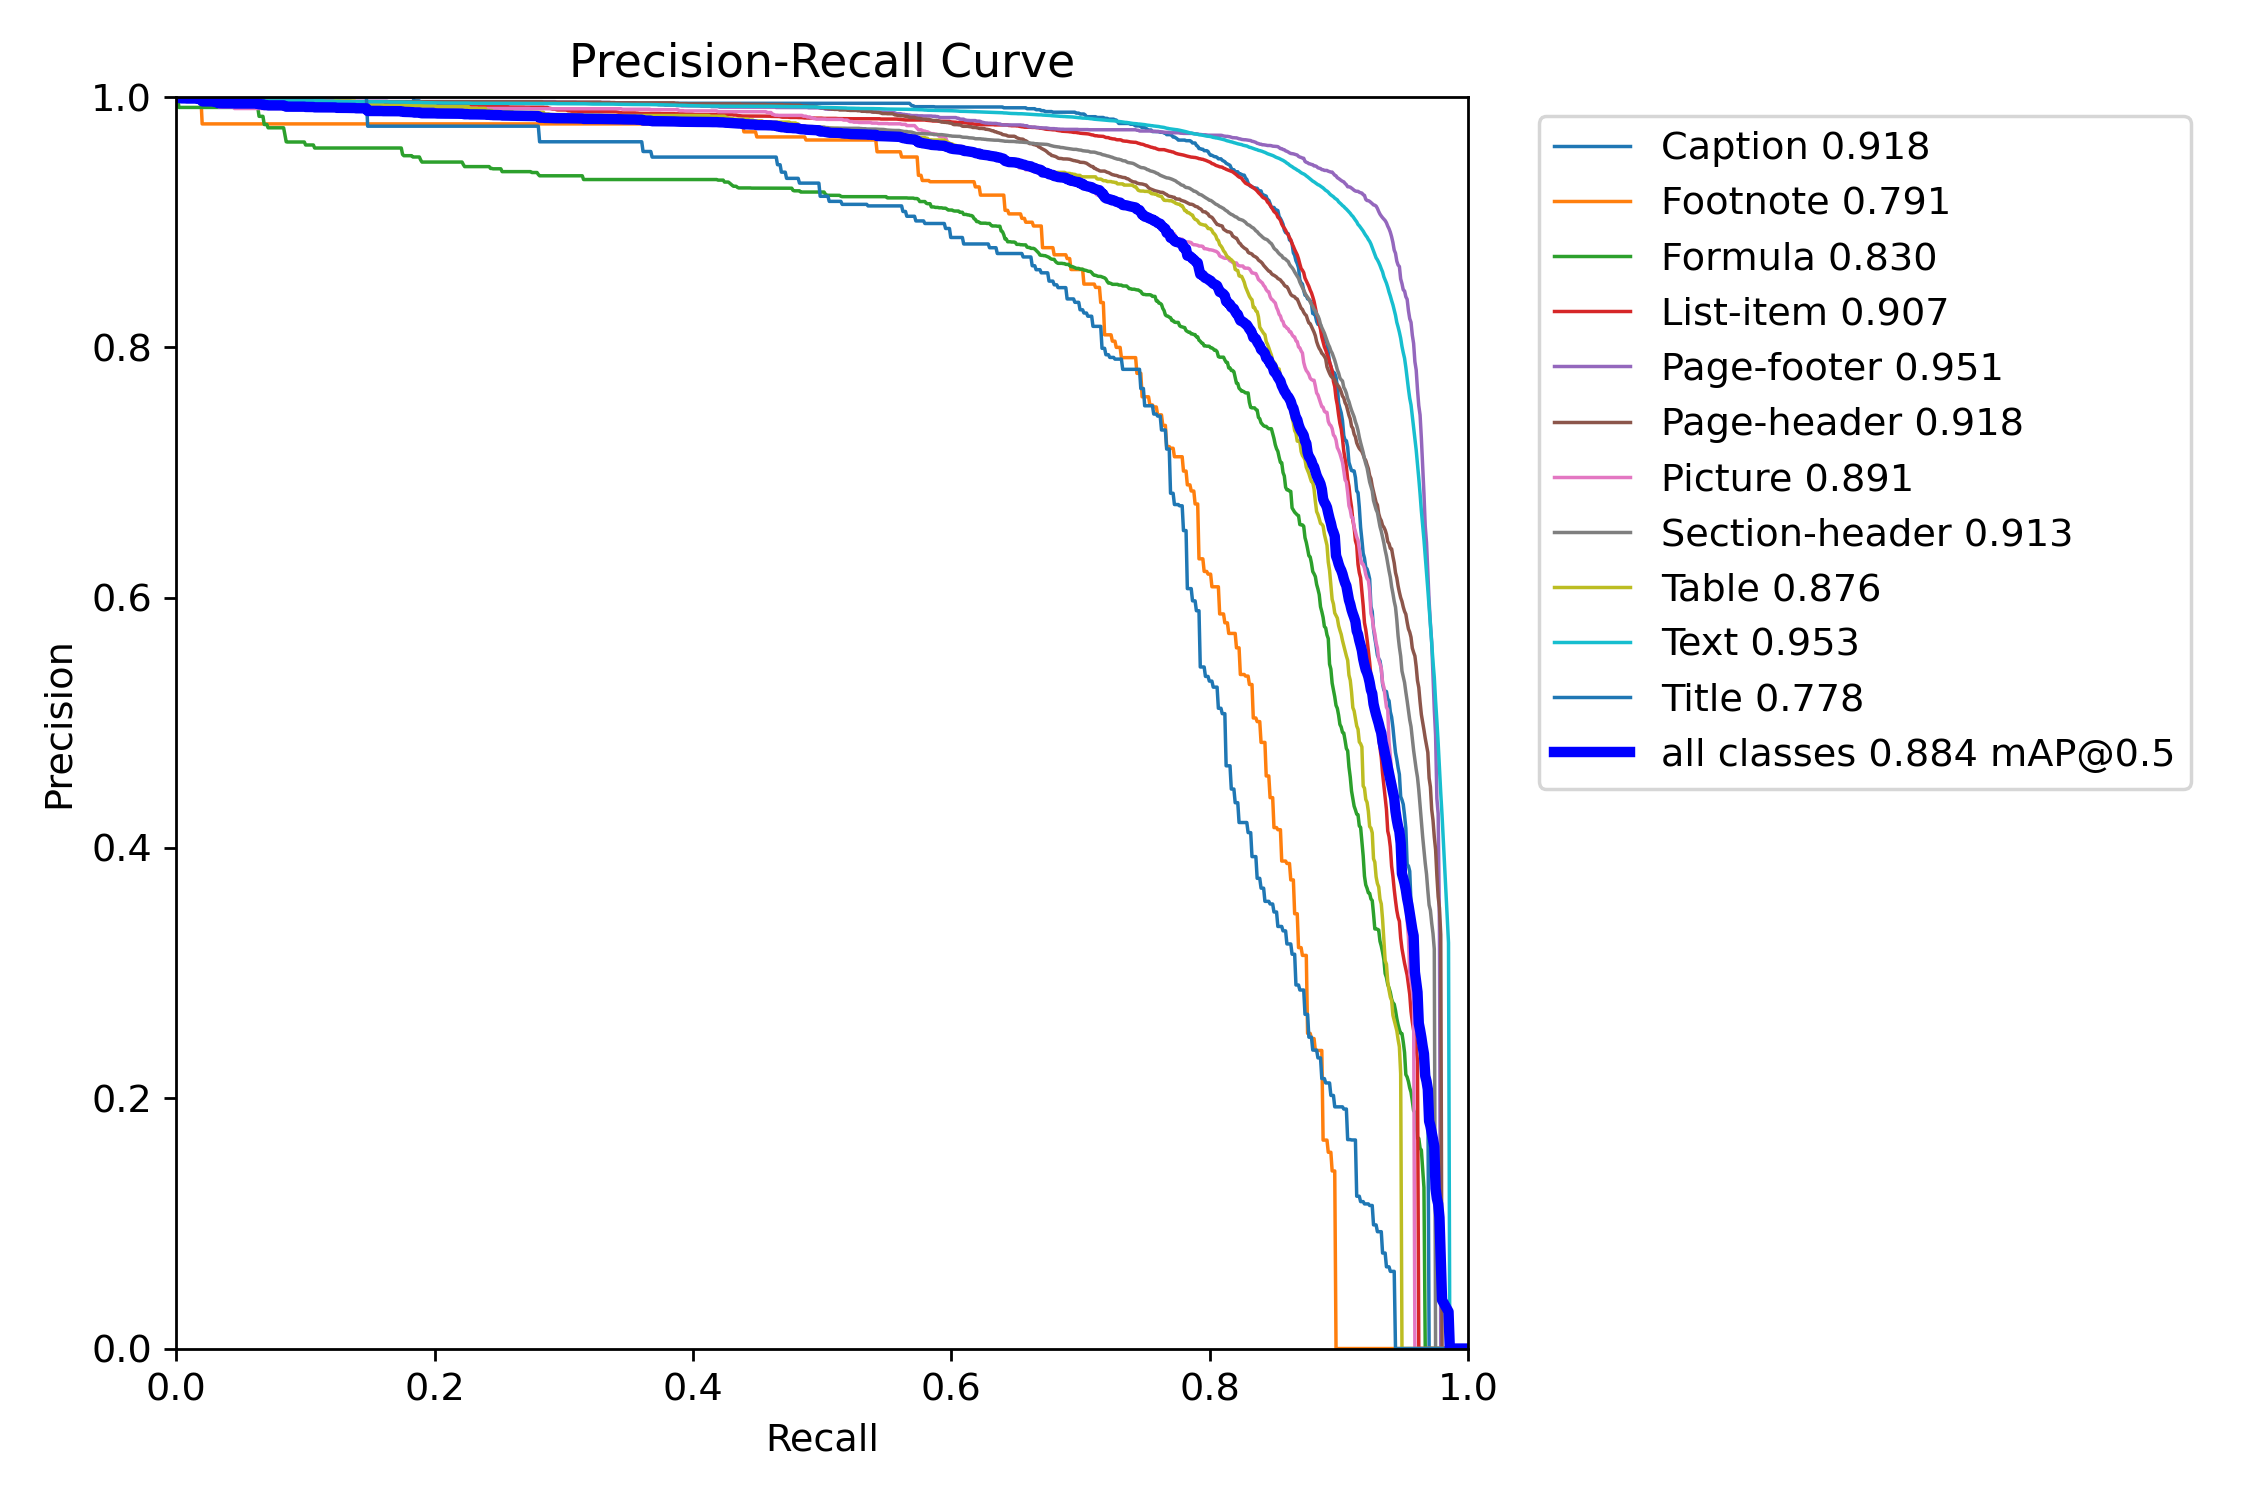
\includegraphics[width=0.92\linewidth]{detection_pr_curve.png}
\caption{Precision-recall curve for the final YOLOv26m detection model.}
\end{figure}

\begin{figure}[H]
\centering
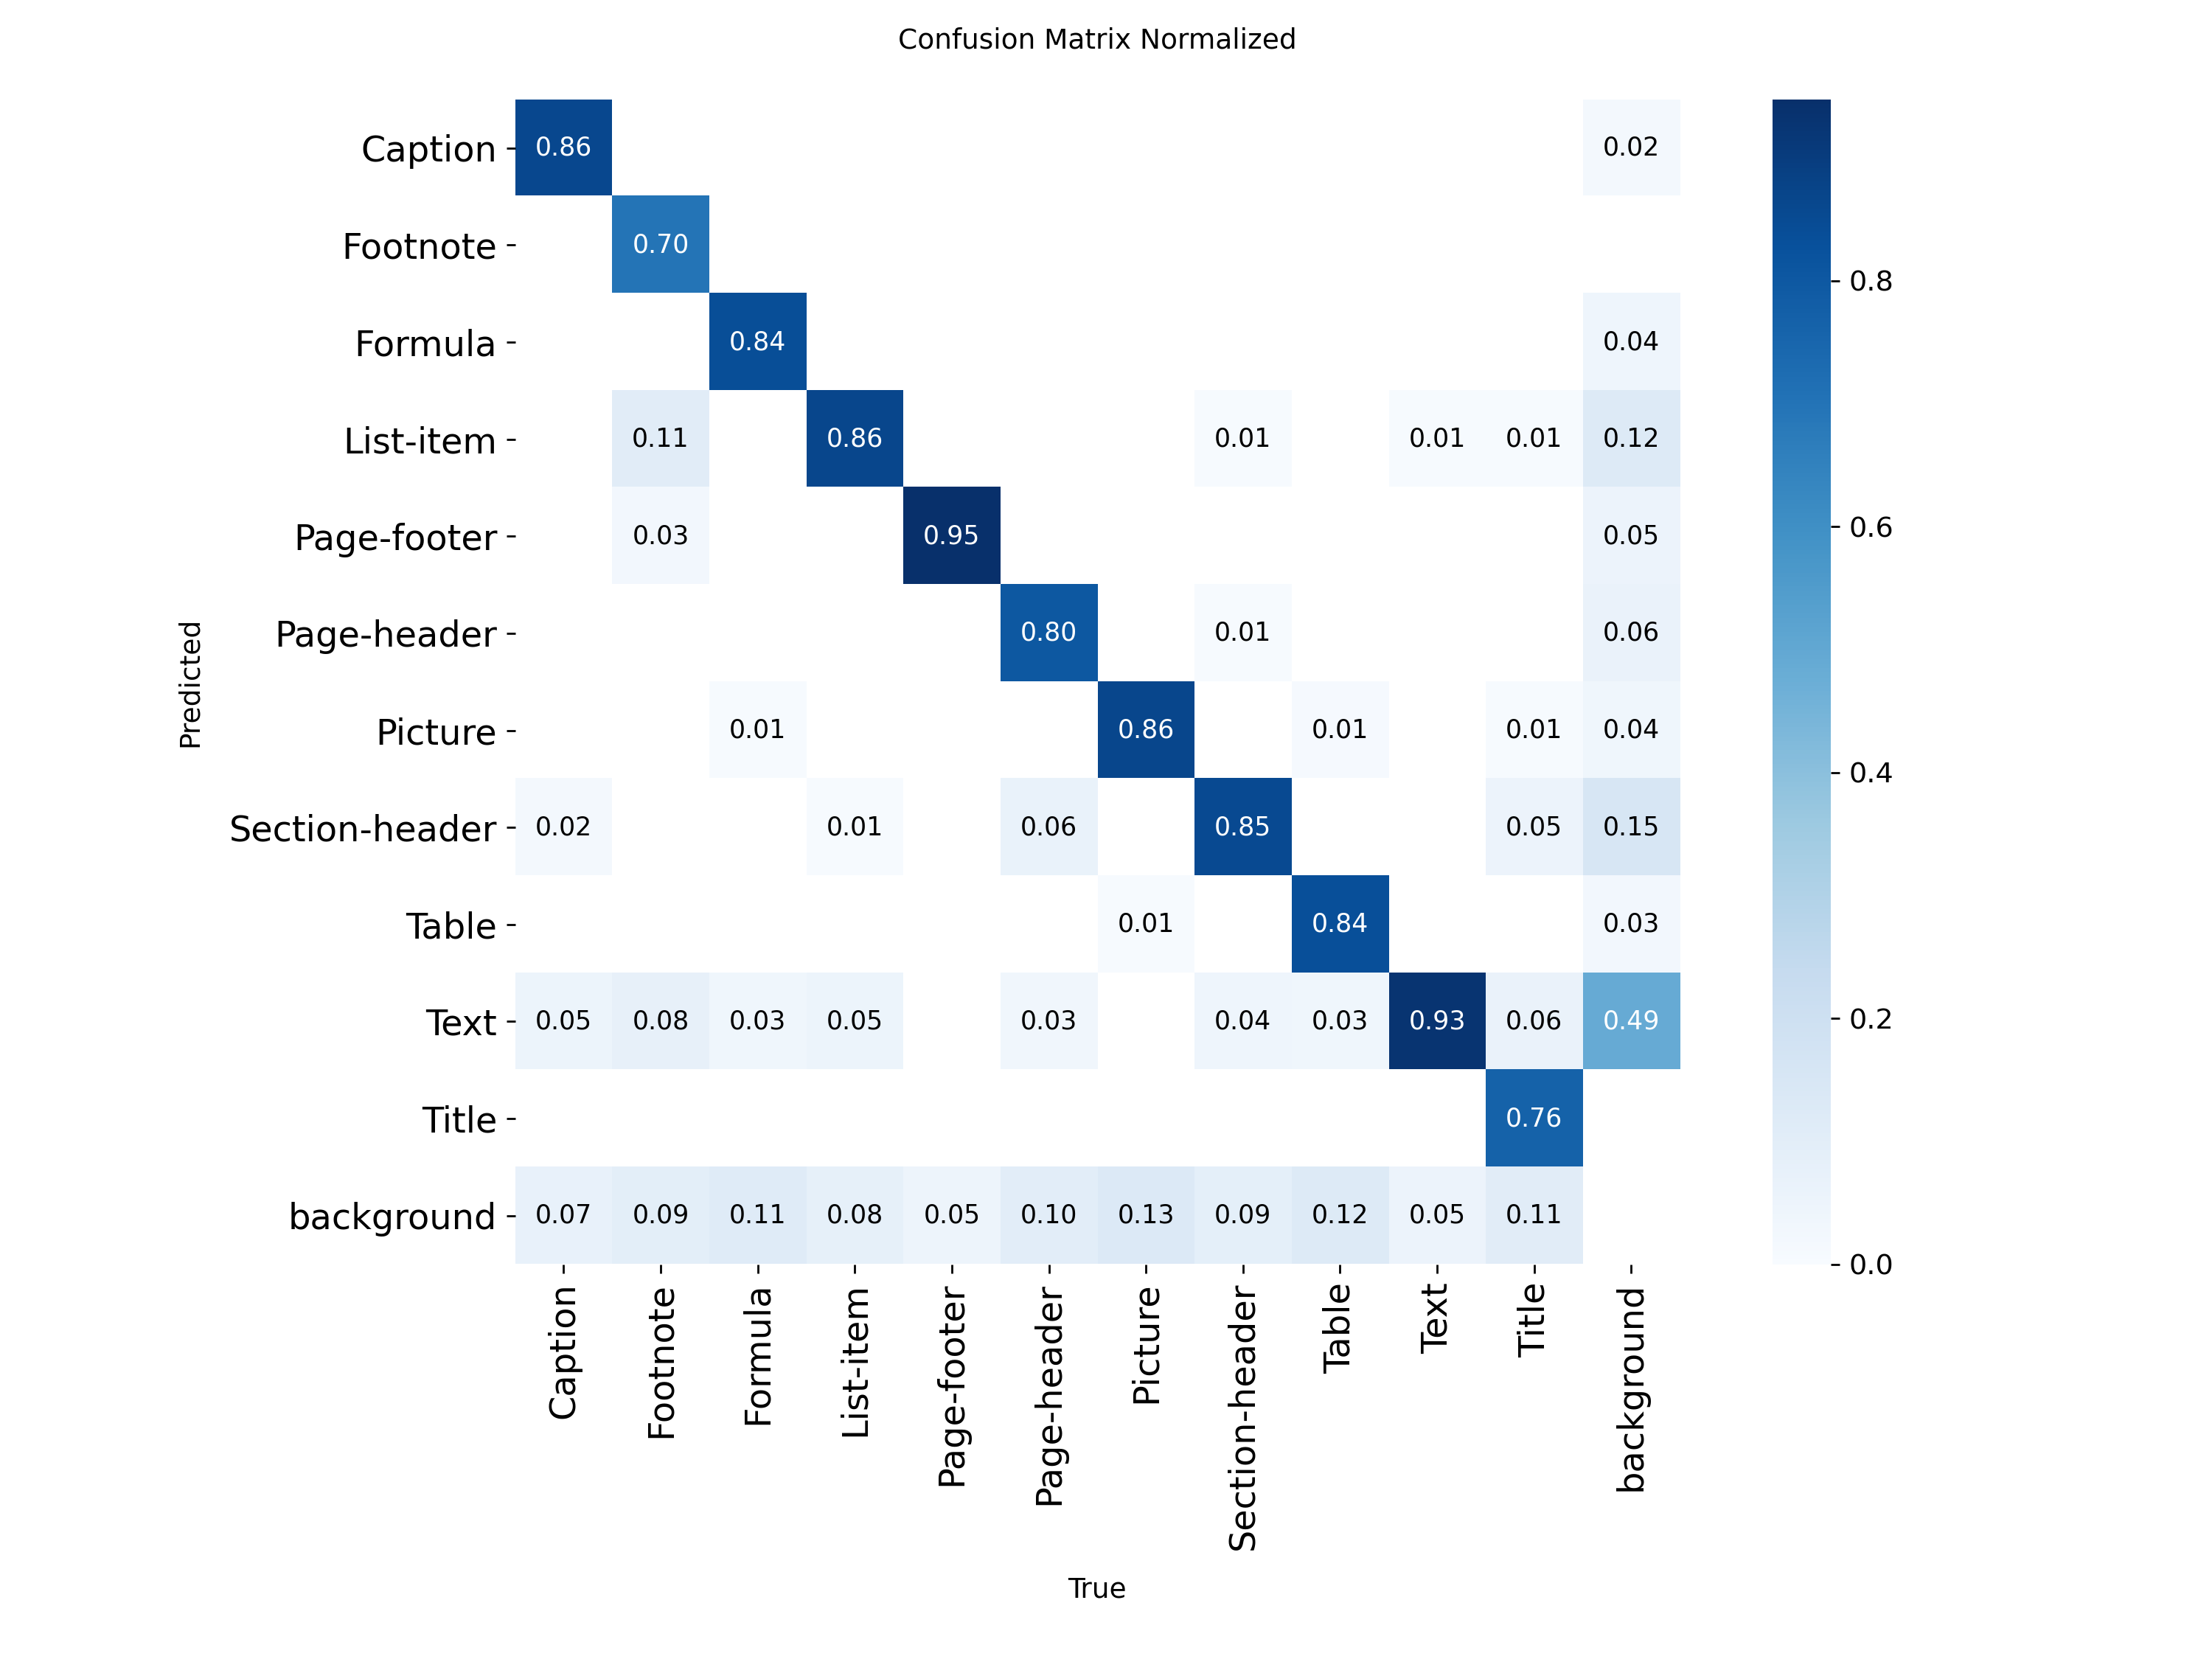
\includegraphics[width=0.92\linewidth]{detection_confusion_matrix_normalized.png}
\caption{Normalized confusion matrix for the final detection validation run.}
\end{figure}

\majorsection{3) Visual Results}

\bluesubsection{Input Page}

The bundled demo page is a scanned financial report page with page headers, section headers, dense paragraphs, and a page footer. This page was kept as the single demo sample because it produces the cleanest end-to-end reconstruction and gives a representative mix of document region types.

\begin{figure}[H]
\centering
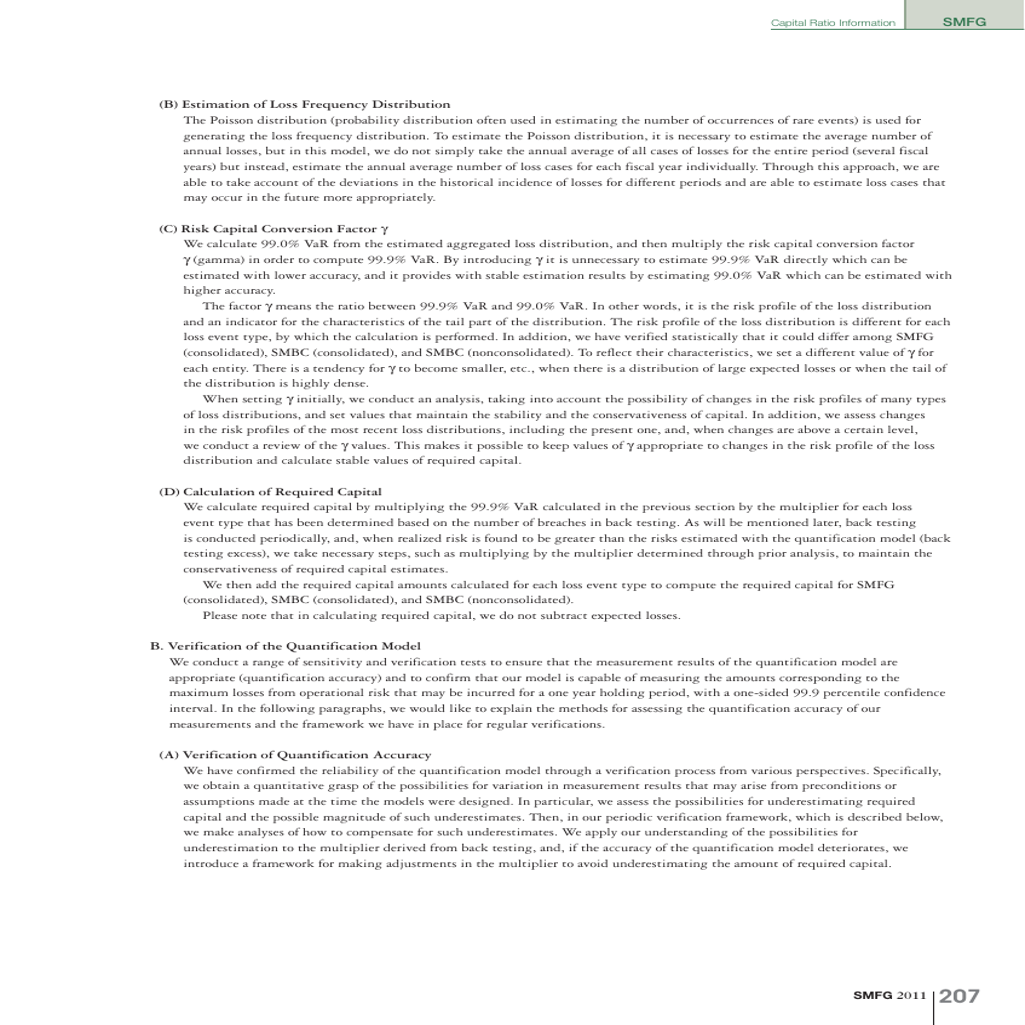
\includegraphics[width=0.78\linewidth,height=0.78\textheight,keepaspectratio]{sample_page.png}
\caption{Bundled sample page used by the final demo.}
\end{figure}

\bluesubsection{YOLO Layout Detection}

The detector identifies the main semantic regions on the page. Orange regions represent normal text blocks, green regions represent section headers, gray regions represent page header/footer material, and other colors mark additional classes.

\begin{figure}[H]
\centering
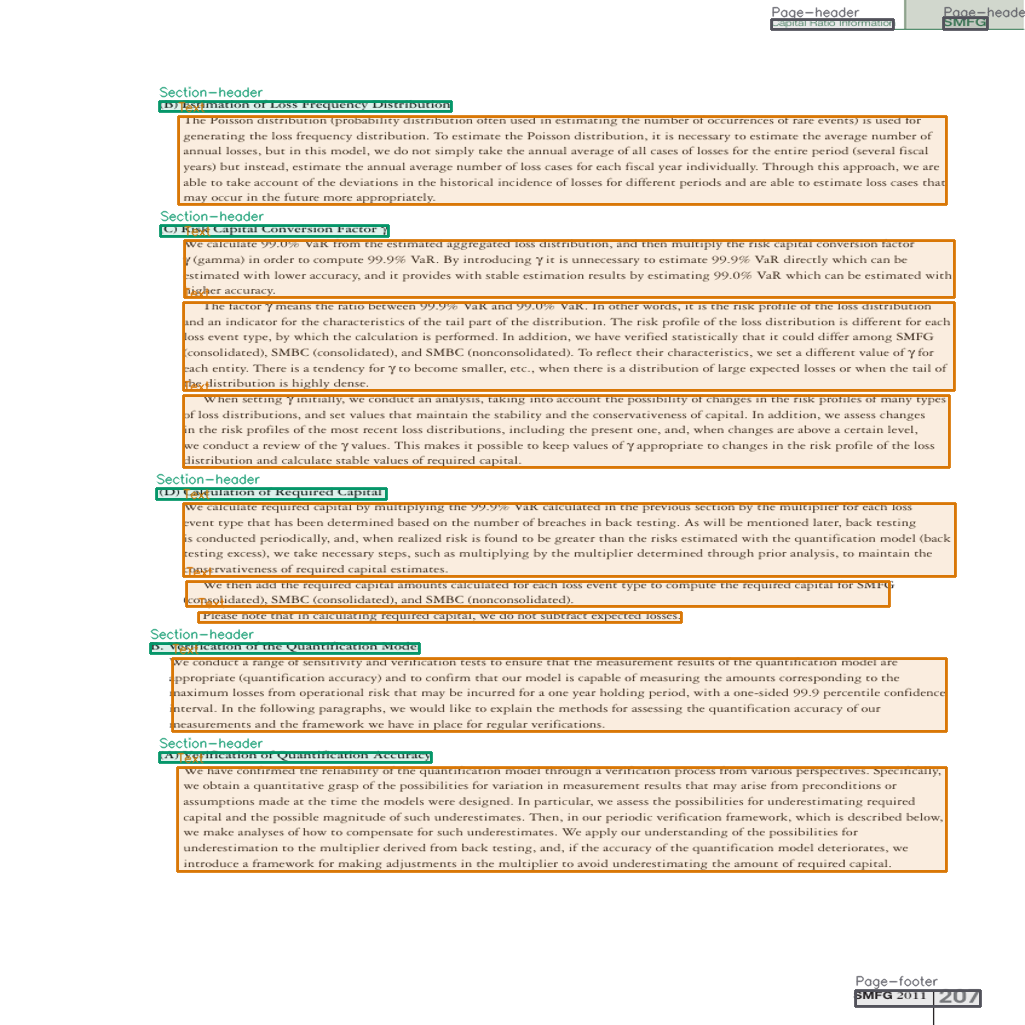
\includegraphics[width=0.78\linewidth,height=0.78\textheight,keepaspectratio]{sample_layout_clean.png}
\caption{Detected layout regions on the bundled sample page.}
\end{figure}

\bluesubsection{Reading Order}

After OCR, the regions are sorted into a top-to-bottom reading order with column-aware geometric grouping. The order numbers in the following image correspond to the sequence used for Markdown rendering.

\begin{figure}[H]
\centering
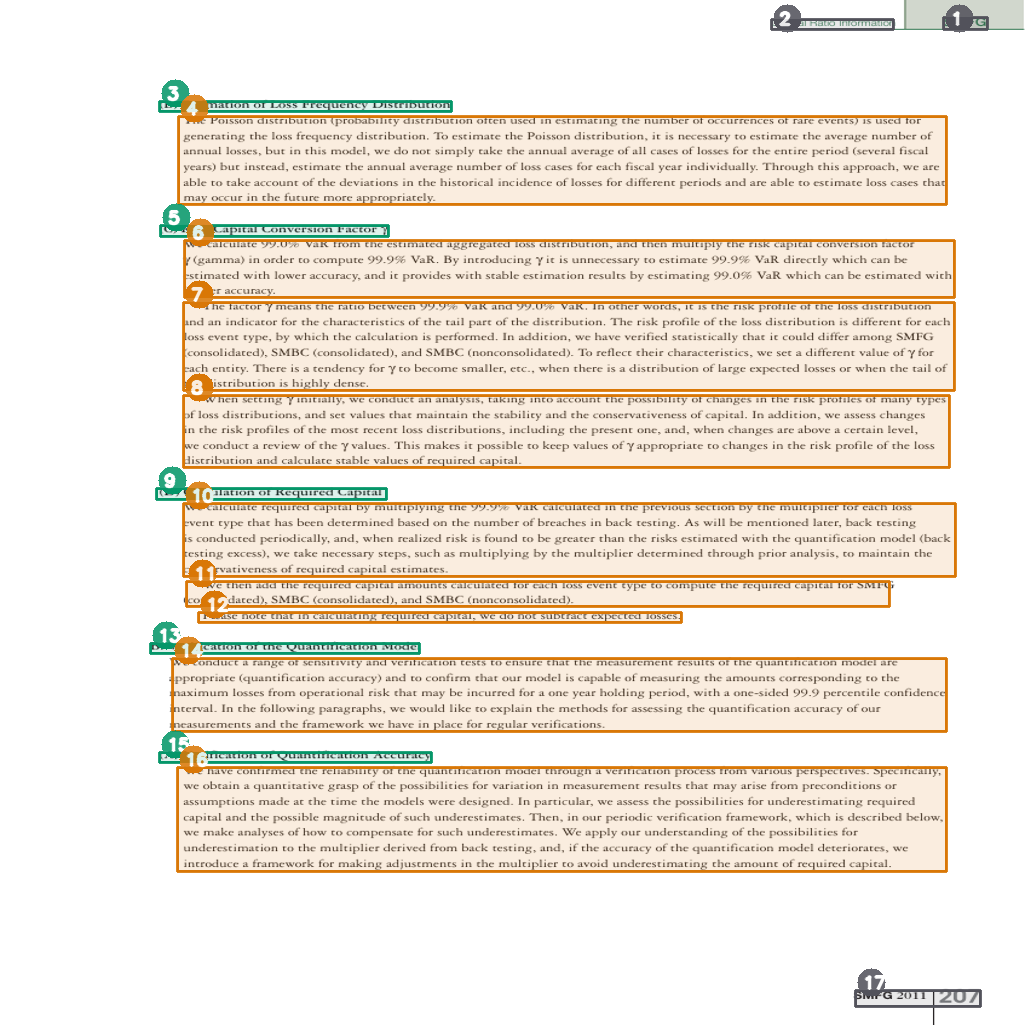
\includegraphics[width=0.78\linewidth,height=0.78\textheight,keepaspectratio]{sample_order_clean.png}
\caption{Reading order assigned to the detected regions.}
\end{figure}

\bluesubsection{Markdown Reconstruction}

The reconstructed Markdown preserves page metadata as comments, converts detected section headers to Markdown headings, and renders paragraph regions as normal text. A representative excerpt from the bundled sample is shown below.

\begin{quote}\small
\texttt{\#\# (B) Estimation of Loss Frequency Distribution}\\
The Poisson distribution is used for generating the loss frequency distribution. To estimate the Poisson distribution, it is necessary to estimate the average number of annual losses, but in this model, we estimate the annual average number of loss cases for each fiscal year individually.\\[0.4em]
\texttt{\#\# (D) Calculation of Required Capital}\\
We calculate required capital by multiplying the 99.9\% VaR calculated in the previous section by the multiplier for each loss event type.
\end{quote}


\majorsection{4) Implementation}

\bluesubsection{Create Training Data}

The dataset conversion scripts transform the DocLayNet-style COCO annotations into YOLO detection and segmentation datasets. The detection dataset stores rectangular boxes, while the segmentation dataset stores polygon masks when available. Both conversions preserve the same semantic class list so that model outputs map directly into Markdown rendering rules.

\bluesubsection{Train and Evaluate Models}

Training is handled through small Python entrypoints around Ultralytics YOLO. The final detection run used YOLOv26m at 1024 pixel resolution, batch size 8, cosine learning rate scheduling, and conservative document augmentations. Validation was then run on the saved best checkpoint to produce precision, recall, mAP50, mAP50-95, PR curves, and a normalized confusion matrix.

\bluesubsection{OCR and Reconstruction}

The OCR stage uses the packaged PP-OCRv6 medium recognition model. Since this is a recognizer, not a detector, wide YOLO crops are split into text lines and chunks before recognition. For table-like crops, long horizontal and vertical ruling lines are removed before row splitting so that table borders do not merge unrelated text rows. Markdown rendering then uses region class names, OCR text, and OCR line geometry to choose headings, paragraphs, lists, tables, figure placeholders, and page metadata comments.

\bluesubsection{Reproducible Demo}

The repository includes one Windows script and one Linux/macOS script. Each script installs \texttt{uv} if needed, runs \texttt{uv sync}, and starts the Streamlit demo. The final YOLO checkpoints and OCR model are included in the repository, so the demo does not require external model downloads during grading.

\majorsection{5) Code}

The project code is available at:

\begin{center}
\Large\url{https://github.com/austinconnor/cap6665-project-1}
\end{center}

\end{document}